\documentclass[12pt,a4paper]{article}
\usepackage[utf8]{inputenc}
\usepackage[spanish]{babel}
\usepackage{amsmath}
\usepackage{amsfonts}
\usepackage{amssymb}
\usepackage{wrapfig}
\usepackage{graphicx}
\usepackage{float}
\usepackage{caption}
\usepackage{hyperref}
\usepackage[left=2cm,right=2cm,top=2cm,bottom=2cm]{geometry}
\usepackage{multicol}
\author{Tatiana Dávila Egas}
\title{Modelo Atómico de Bohr}
\date{}
\begin{document}
\maketitle
\tableofcontents

\section{Modelo atómico de Bohr} 
El modelo atómico de Bohr o de Bohr-Rutherford es un modelo clásico del átomo, pero fue el primer modelo atómico en el que se introduce una cuantización a partir de ciertos postulados. Fue propuesto en 1913 por el físico danés Niels Bohr,2 para explicar cómo los electrones pueden tener órbitas estables alrededor del núcleo y por qué los átomos presentaban espectros de emisión característicos (dos problemas que eran ignorados en el modelo previo de Rutherford). Además el modelo de Bohr incorporaba ideas tomadas del efecto fotoeléctrico, explicado por Albert Einstein en 1905.
\begin{figure}[!ht]
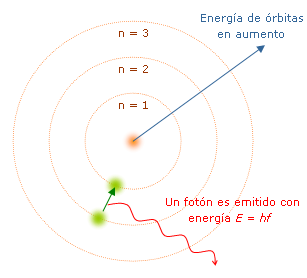
\includegraphics[scale=0.6]{Modelo_de_Bohr.png}
\centering 
\caption{Diagrama del modelo\\ atómico de Bohr}
\end{figure}

\section{Introducción} 

Bohr se basó en el átomo de hidrógeno para hacer el modelo que lleva su nombre. Bohr intentaba realizar un modelo atómico capaz de explicar la estabilidad de la materia y los espectros de emisión y absorción discretos que se observan en los gases. Describió el átomo de hidrógeno con un protón en el núcleo, y girando a su alrededor un electrón. El modelo atómico de Bohr partía conceptualmente del modelo atómico de Rutherford y de las incipientes ideas sobre cuantización que habían surgido unos años antes con las investigaciones de Max Planck y Albert Einstein.

En este modelo los electrones giran en órbitas circulares alrededor del núcleo, ocupando la órbita de menor energía posible, o la órbita más cercana posible al núcleo. El electromagnetismo clásico predecía que una partícula cargada moviéndose de forma circular emitiría energía por lo que los electrones deberían colapsar sobre el núcleo en breves instantes de tiempo. Para superar este problema Bohr supuso que los electrones solamente se podían mover en órbitas específicas, cada una de las cuales caracterizada por su nivel energético. Cada órbita puede entonces identificarse mediante un número entero n que toma valores desde 1 en adelante. Este número "n" recibe el nombre de número cuántico principal.

Bohr supuso además que el momento angular de cada electrón estaba cuantizado y sólo podía variar en fracciones enteras de la constante de Planck. De acuerdo al número cuántico principal calculó las distancias a las cuales se hallaba del núcleo cada una de las órbitas permitidas en el átomo de hidrógeno. Estos niveles en un principio estaban clasificados por letras que empezaban en la "K" y terminaban en la "Q". Posteriormente los niveles electrónicos se ordenaron por números. Cada órbita tiene electrones con distintos niveles de energía obtenida que después se tiene que liberar y por esa razón el electrón va saltando de una órbita a otra hasta llegar a una que tenga el espacio y nivel adecuado, dependiendo de la energía que posea, para liberarse sin problema y de nuevo volver a su órbita de origen. Sin embargo no explicaba el espectro de estructura fina que podría ser explicado algunos años más tarde gracias al modelo atómico de Sommerfeld. Históricamente el desarrollo del modelo atómico de Bohr junto con la dualidad onda-corpúsculo permitiría a Erwin Schrödinger descubrir la ecuación fundamental de la mecánica cuántica.

\section{Postulados de Bohr}

\addcontentsline{toc}{subsection}{Primer postulado}
\subsection*{Primer postulado}
Los electrones describen órbitas circulares en torno al núcleo del átomo sin irradiar energía.

La causa de que el electrón no irradie energía en su órbita es, de momento, un postulado, ya que según la electrodinámica clásica una carga con un movimiento acelerado debe emitir energía en forma de radiación.

Para mantener la órbita circular, la fuerza que siente el electrón —la fuerza coulombiana por la presencia del núcleo— debe ser igual a la fuerza centrípeta. Esto nos da la siguiente expresión:

\begin{equation}
r=k\dfrac{Ze^{2}}{m_{e}v^{2}}
\end{equation}
Y ahora, con esta ecuación, y sabiendo que la energía total es la suma de las energías cinética y potencial:
\begin{equation}
E=T+V=\dfrac{1}{2}m_{e}v^{2}-k\dfrac{Ze^{2}}{r}=-\dfrac{1}{2}\dfrac{kZe^{2}}{r}
\end{equation}
Donde queda expresada la energía de una órbita circular para el electrón en función del radio de dicha órbita.

\addcontentsline{toc}{subsection}{Segundo postulado}
\subsection*{Segundo postulado}

\begin{multicols}{2}
No toda órbita para electrón está permitida, tan solo se puede encontrar en órbitas cuyo radio cumpla con el momento angular, $L$, del electrón sea un múltiplo entero de $\hbar=\dfrac{h}{2\pi}$. Esta condición matemáticamente se escribe: $$L=m_{e}vr=n\hbar$$ con $n= 1,2,3...$.\\ A partir de ésta condición y de la expresión para el radio obtenida antes, podemos eliminar $v$ y queda la condición de cuantización para los radios permitidos:
$$r_{n}=\dfrac{n^{2}\hbar^{2}}{km_{e}Ze^{2}}$$ con $n= 1,2,3\ldots$  \ ; subíndice introducido     en esta expresión para resaltar que el radio ahora es una magnitud discreta, a diferencia de lo que decía el primer postulado.

Ahora, dándole valores a $n$, número cuántico principal, obtenemos los radios de las órbitas permitidas. Al primero de ellos (con n=1), se le llama radio de Bohr:
$$a_{0}=\dfrac{\hbar^{2}}{km_{e}e^{2}}=0.52$$
expresando el resultado en \aa ngstr\"om.\\

\begin{center}
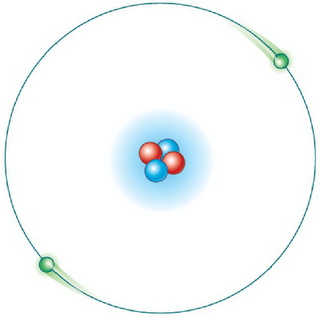
\includegraphics[scale=.4]{MODELO_ATOMICO_DE_BOHR2pos.png}
\end{center}


Del mismo modo podemos ahora sustituir los radios permitidos $r_n$ en la expresión para la energía de la órbita y obtener así la energía correspondiente a cada nivel permitido:
$$E_n=-\dfrac{1}{2}\dfrac{k^2m_eZ^2e^4}{n^2\hbar^2}$$
Igual que antes, para el átomo de hidrógeno $(Z=1)$ y el primer nivel permitido $(n=1)$, obtenemos:
$$E_0=-\dfrac{1}{2}\dfrac{k^2m_{e}e^4}{hbar^2}=-13.6eV$$
que es la llamada energía del estado fundamental del átomo de Hidrógeno.

Y podemos expresar el resto de energías para cualquier $Z$ y $n$ como:
$$E_n=\dfrac{Z^2}{n^2}E_0$$

\end{multicols}

\addcontentsline{toc}{subsection}{Tercer postulado}
\subsection*{Tercer postulado}

\begin{multicols}{2}

\begin{center}
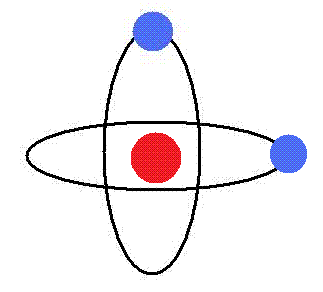
\includegraphics[scale=0.5]{Bohr-model3pos.png} 
\end{center}
El electrón solo emite o absorbe energía en los saltos de una órbita permitida a otra. En dicho cambio emite o absorbe un fotón cuya energía es la diferencia de energía entre ambos niveles. Este fotón, según la ley de Planck tiene una energía: $$E_{\gamma}=hv=E_{nf}-E_{ni}$$ 
donde $n_i$ identifica la órbita inicial y $n_f$ la final, y $\nu$ es la frecuencia.\\
Entonces las frecuencias de los fotones emitidos o absorbidos en la transición serán:
$$v=\dfrac{k^{2}m_{e}Z^{2}e^{4}}{2h\hbar^{2}}\left( \dfrac{1}{n^{2}_i}-\dfrac{1}{n^{2}_{i}}\right)$$
Se puede demostrar que este conjunto de hipótesis corresponde a la hipótesis de que los electrones estables orbitando un átomo están descritos por funciones de onda estacionarias. Un modelo atómico es una representación que describe las partes que tiene un átomo y como están dispuestas para formar un todo. Basándose en la constante de Planck $E=hv$, consiguió cuantizar las órbitas observando las líneas del espectro.

\end{multicols}

\addcontentsline{toc}{subsection}{Representación de las órbitas}
\subsection*{Representación de las órbitas}
\begin{center}
  \begin{tabular}{ | c | c | c | }
    \hline
    Diagrama & n & Distancias \\ \hline
    \begin{minipage}{.3\textwidth}
    \centering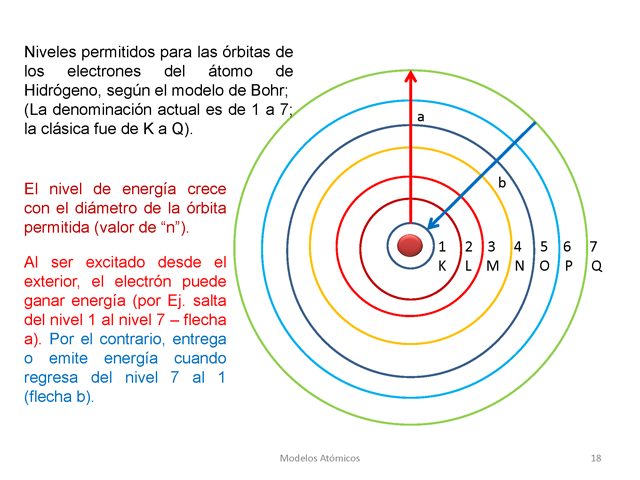
\includegraphics[scale=0.65]{orbitas}
    \end{minipage}
    &
    \begin{minipage}[c]{6cm}
      \begin{itemize}
        \item 1
        \item 2
        \item 3
        \item 4
        \item 5
        \item 6
        \item 7
      \end{itemize}
    \end{minipage}
    & 
    \begin{minipage}[c]{6cm}
      \begin{itemize}
        \item 0.53 A
        \item 2.12 A
        \item 4.76 A
        \item 8.46 A
        \item 13.22 A
        \item 19.05 A
        \item 25.93 A
      \end{itemize}
    \end{minipage}
    \\ \hline
  \end{tabular} 
\end{center}


\section{Temas Relacionados}

\begin{itemize}
\item Modelo atómico de Dalton
\item Modelo atómico de Thompson
\item Modelo atómico de Rutherford
\item Modelo atómico de Sommerfeld
\item Modelo atómico de Schr\"odinger
\end{itemize}

\section{Bibliografía}
\href{<https://es.wikipedia.org/wiki/Modelo_at\%C3\%B3mico_de_Bohr>}{Wikipedia}

\end{document}